\section{Evaluation \& Results} 
			
\begin{frame}[shrink]{Evaluation and Results Overview}

\begin{block}{Objective}
    Evaluate \alert{model generalization on unseen data} using standardized 
    financial forecasting metrics.
\end{block}

\vspace{0.5em}

\begin{block}{Evaluation Metrics}
\begin{itemize}
    \item \textbf{Root Mean Squared Error (RMSE)}: Penalizes large prediction errors heavily.
    \item \textbf{Mean Absolute Error (MAE)}: Measures the average size of errors.
    \item \textbf{Coefficient of Determination ($R^2$)}: Captures goodness of fit (variance explained).
    \item \textbf{Mean Absolute Percentage Error (MAPE)}: Provides scale-independent, percentage-based
    error.
\end{itemize}
\end{block}

\note{
We assess models using four widely accepted metrics to get a complete picture of their predictive 
ability.
This helps ensure robust comparison and validates the model's effectiveness for stock price forecasting.
}
\end{frame}

\begin{frame}[shrink]{Test Set Evaluation Results}

\begin{block}{Evaluation Setup}
    \begin{itemize}
        \item Models evaluated on completely unseen test data (2014–2025).
        \item Predictions inverse-transformed to real price scale using the training MinMaxScaler.
        \item Metrics computed to assess generalization to future stock price movements.
    \end{itemize}
\end{block}

\vspace{0.8em}

\begin{block}{Performance on Test Dataset}
\centering
\begin{tabular}{lcccc}
\hline
\textbf{Model} & \textbf{RMSE} & \textbf{MAE} & \textbf{MAPE} & \textbf{R\textsuperscript{2}} \\
\hline\hline
LSTM & 5.1674 & 4.1259 & 4.88\% & 0.9455 \\
\textbf{LSTM-BiGRU} & \textbf{1.9980} & \textbf{1.3178} & \textbf{1.27\%} & \textbf{0.9919} \\
\hline
\end{tabular}
\end{block}

\note{
Both models generalized well to unseen data, but LSTM-BiGRU significantly outperformed LSTM across all metrics.
It halved the RMSE and MAE, achieved an R\textsuperscript{2} above 0.99, and maintained a very low MAPE, confirming stronger forecasting accuracy.
}
\end{frame}

\begin{frame}[shrink]{Visual Results Comparison: Actual vs Predicted Prices}
\centering
\resizebox{1.3\linewidth}{!}{%
\begin{tabular}{m{2cm}m{10cm}}
    \textbf{LSTM} & 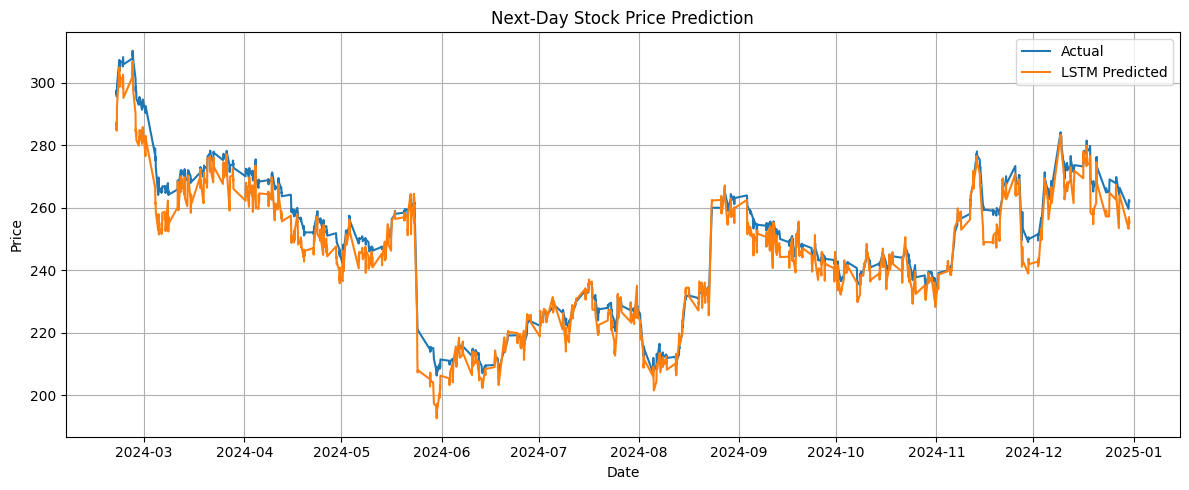
\includegraphics[width=0.7\textwidth]{img/main/pred-lstm.png} \\
    \textbf{LSTM-BiGRU} & 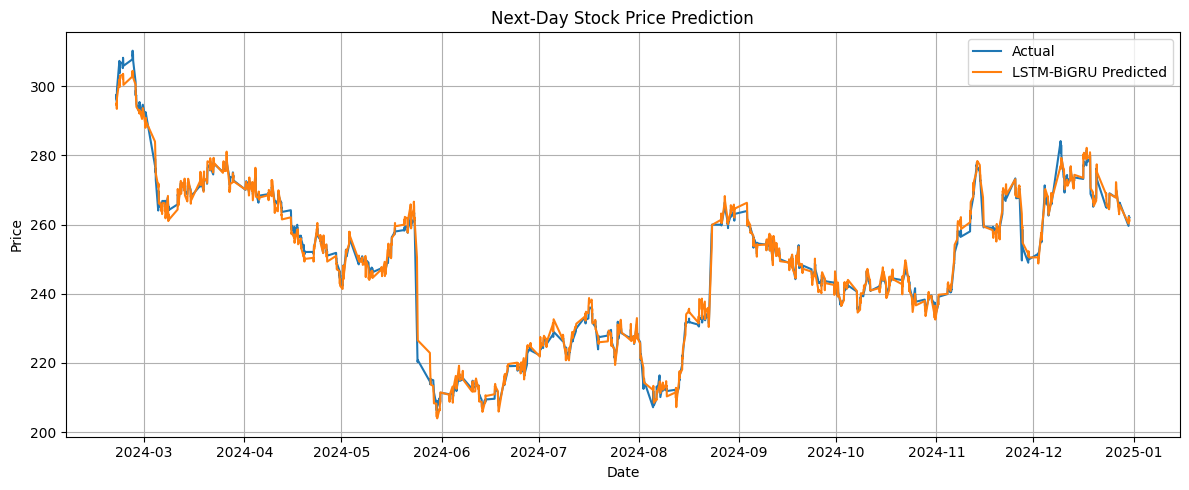
\includegraphics[width=0.7\textwidth]{img/main/pred-bigru.png} \\
\end{tabular}
}
\note{
The top chart shows all models together. The lower charts show individual comparisons.
LSTM-BiGRU follows the actual price more closely, especially during periods of volatility.
The standalone LSTM shows slightly more deviation and smoothing of sharp price movements.
}
\end{frame}
